
\chapter{White noise based algorithms for modeling Gaussian random processes}
\label{Chapter:White noise based algorithms for modeling Gaussian random processes}
    Observable sources are those that composed from many contributions and as the number of contributors growths it's not possible the define this sources deterministically. At this point Statistical optic theory is a perfect language for describing the behaviour of electron magnetic fields from real life sources.

    There are many examples of radiation sources the are random by its nature: starts, light bulbs or thermal sources, SR and FEL radiation etc. As to my own experience not many fundamental text books sires include description of statistical optical phenomena, e.g. famous sires written by L. Landau and E. Lifshitz covers only basics of optical theory, R. Feiman also… Dedicated textbooks on statistical optics are usually referred to graduate students which already implies for those who already have had chosen their specialization on the topic and not for broader audience of students in physics. 

    Important role play Gaussian random processes…

    There are several methods for simulating statistical optics phenomena…

    In the chapter I present a set of methods for simulating Gaussian random fields based on a computationally efficient algorithm…

    Introducing this methods necessitate outlining basics of statistical optics theory. I start with general definitions of a random processes and treir properties. I will dive in the concept of stationary and ergodicity and intoruce the definition Gaussian random processes. Then I outline the theory for quasi-stationery sources in the very similar manner that have been done in~\cite{wolgoodman_statistical_2015} and proofs more general form of Wiener-Khinchin theorem. Having this I start to consider transverce coherence properties of raidiation and provide derivation for the generilized van Cittert-Zernike theorem. After this I discuss methods for simulating synchrotron radiation, and then I present the white-noise based methods for simulating partially coherent radiation. These method are presented at first with heuristic consideration and then each method is presented in application to simulation problem: bending magnet radiation, undulator radiation, FEL SASE radiation 
    
\section{Classification of random processes}
    Statistical realizations is a "one of roll of the dice" of the statistical process, meaning that an observer recorded the process over some time interval $[-T/2, T/2]$ within which the process happened. This realization, let's say is $k$-th realization of the process $U$ and one can find the average integrating over time:
    \begin{align}
        \overline{u^{[k]}(t)} = \frac{1}{T} \int \limits_{t - T/2}^{t + T/2}  u^{[k]}(t') dt',
        \label{Eq:time_avr}
    \end{align}
    here I used the definition presented in~\oo{Mendel Wolf}.
    and the for the second moment or \textit{time auto-correlation function}
    \begin{align}
        \overline{u(t_1)u(t_2)} = \frac{1}{T} \int \limits_{t - T/2}^{t + T/2} u^{[k]}(t + t_1)u^{[k]}(t + t_2)dt
        \label{Eq:time_autocorrelation}
    \end{align}

    As we deal with random processes we can define, surely for each point of time $t_i$ for each realization $u_k(t_i)$ is a random variable with a set of probability density functions $p(u, t_i)$, which depend both on time and on the chosen realization. Unfortunately, to fully describe statistical process one need to know not only $p(u, t_i)$ - the first order probability density function does not describe process fully as does not contain any information about correlation happening between $t_1, t_2, …, t_n$, where in principal $n$ should be equal infinity. So, on need to know subsequently second order moment $p_2(u_1, t_1, u_2, t_2)$ and up to $n$-th order joint probability density function $p_n(u_1, t_1, u_2, t_2, …u_n, t_n)$. In the next chapter I will introduce the type of the process called Gaussian, where the process could be full define with only knowing the first and the second order probability density function.

    With probability density function I can define another time of averaging: ensamble averaging:
    \begin{align}
        \langle u(t) \rangle = \int u p(u, t) dx,
        \label{Eq:ensemble_int_avr}
    \end{align}
    and for the second order:
    \begin{align}
        \Gamma(t_1, t_2) = \langle u(t_1)u(t_2) \rangle = \iint u_1u_2 p_2(u_1, t_1, u_2, t_2) du_1du_2,
        \label{Eq:ensemble_int_autocorrelation}
    \end{align}
    but most of the time on practice it is not possible to know $p(u, t)$ and its high order colleagues, and there is another useful definition. If one collected reasonably large statistical ensemble: $u^{[1]}(t), u^{[2]}(t), …, u^{[k]}(t)$, then statistical average can be defined as the following:
    \begin{align}
        \langle u(t) \rangle = \lim_{N\to\infty} \frac{1}{N}\sum_{i=1}^{N} u^{[i]}(t)
        \label{Eq:ensemble_avr}
    \end{align}
    and the second order auto-correlation function:
    \begin{align}
        \Gamma(t_1, t_2) = \langle u(t_1)u(t_2) \rangle = \lim_{N\to\infty} \frac{1}{N}\sum_{i=1}^{N} u^{[i]}(t_1)u^{[i]}(t_2)
        \label{Eq:ensemble_autocorrelation}
    \end{align}
    The definitions are fully equivalent to Eq.~\ref{Eq:ensemble_int_avr} and~\ref{Eq:ensemble_int_autocorrelation} and are much more usefully, as only requires measurement of the realizations itself without any \textit{a priori} knowledge about the process. In this thesis I will mostly rely on the later to definitions and its higher order \rr{colleagues}.
    
    \subsection{Stationarity and ergodicity}
    In this section I will introduce two important concepts of statistical optics: stationarity and ergodicity. The later one relates definition of time average given by Eq.~\ref{Eq:time_avr} and~\ref{Eq:time_autocorrelation} with average over realizations given by Eq.~\ref{Eq:ensemble_avr} and Eq.~\ref{Eq:ensemble_autocorrelation} or its integral analogues. 
    
    As soon as I introduced probability density function distributions I can define condition for the process to be stationary.
    \begin{align}
        p_n(u_1, t_1, u_2, t_2, …u_n, t_n) = p_n(u_1, t_1 + T, u_2, t_2 + T, …u_n, t_n + T) \; \textup{for all} \; T
        \label{Eq:stationary_strict}
    \end{align}
    As the chose of $T$ is arbitrary we can set it to be one of $t_n$ variables and find that for example autocorrelation function depended only on time difference  $\Delta t = t_2 - t_1$.
    \begin{align}
        \Gamma(t_1, t_2) = \lim_{N\to\infty} \frac{1}{N}\sum_{i=1}^{N} u^{[i]}(t)u^{[i]}(t + t_2 - t_1) = \langle u(t)u(t + t_2 - t_1) \rangle
    \end{align}
    for all $t$ values.
    
    The definition by Eq.~\ref{Eq:stationary_strict} is quite strict, it is also called \textit{strict-sense stationarity} and in practice usually look at the dependence on $t$ of the average and the first order correlation function, if they do not depend on $t$ and the first order correlation function depends only on time difference  $\Delta t$ then the process is called \textit{wide-sense stationary}.

    As one can see in statistical optics there are two conceptual ways to define averages: over time and across different realizations. In general, these averages are different but there is a specific time of the process for which these two averages are equivalent. This type of the process are \textit{ergodic} and writing its definition explicitly:
    \begin{align}
        \lim_{N\to\infty} \frac{1}{N}\sum_{i=1}^{N} u^{[i]}(t) = \frac{1}{T} \int \limits_{t - T/2}^{t + T/2}  u^{[k]}(t') dt'
    \end{align} 
    for any $t$, $T$ and taken $k$-th realization of the process. And the same can be written for the autocorrelation function:
    \begin{align}
        \lim_{N\to\infty} \frac{1}{N}\sum_{i=1}^{N} u^{[i]}(t_1)u^{[i]}(t_2) = \frac{1}{T} \int \limits_{t - T/2}^{t + T/2} u^{[k]}(t + t_1)u^{[k]}(t + t_2)dt
    \end{align}
    again for any $t$, $T$ and taken $k$-th realization. This definition is very mathematically elegant and very useful in many applications \oo{where?}

    The type of the process I have described are fundamental for statistical optics but surely cannot describe all the observed process while the mathematical language can be adapted or extended to more general cases. 

    \subsection{Gaussian random processes}

    Gaussian random process play the pivotal role in statistical optics. Although there are numerous exclusion overall one can notice that in physical systems processes are composed from many individual additive contributions, which, accounting for the central limit theorem, leads to Gaussian statistics of the processes. Expressing this kind of statistics in mathematical term I start with definition for the probability density function for a random process $x$:
    \begin{align}
        p(x) = \cfrac{1}{\sqrt{2 \pi}\sigma} e^{-x^2/2\sigma^2},
    \end{align}
    where $\sigma$ is the dispersion of a random process $x$.
    As it is always convenient to work with analytic representation of a signal I introduce here a very definition of the circular complex Gaussian random processes: $z = x + iy$, both process has the same value of dispersion.
    \begin{align}
        p(z) = p(x)p(y) = \cfrac{1}{\sqrt{2 \pi}\sigma} e^{-(x^2 + y^2)/2\sigma^2},
    \end{align}
    which can be transformed to using polar coordinates $x = A\cos(\phi)$ and $y = A\sin(\phi)$:
    \begin{align}
        p(z) = p(A, \phi) = \cfrac{A}{\sqrt{2 \pi}\sigma} e^{-A^2/2\sigma^2}.
    \end{align}
    \begin{figure}[h!]
    	\centering
        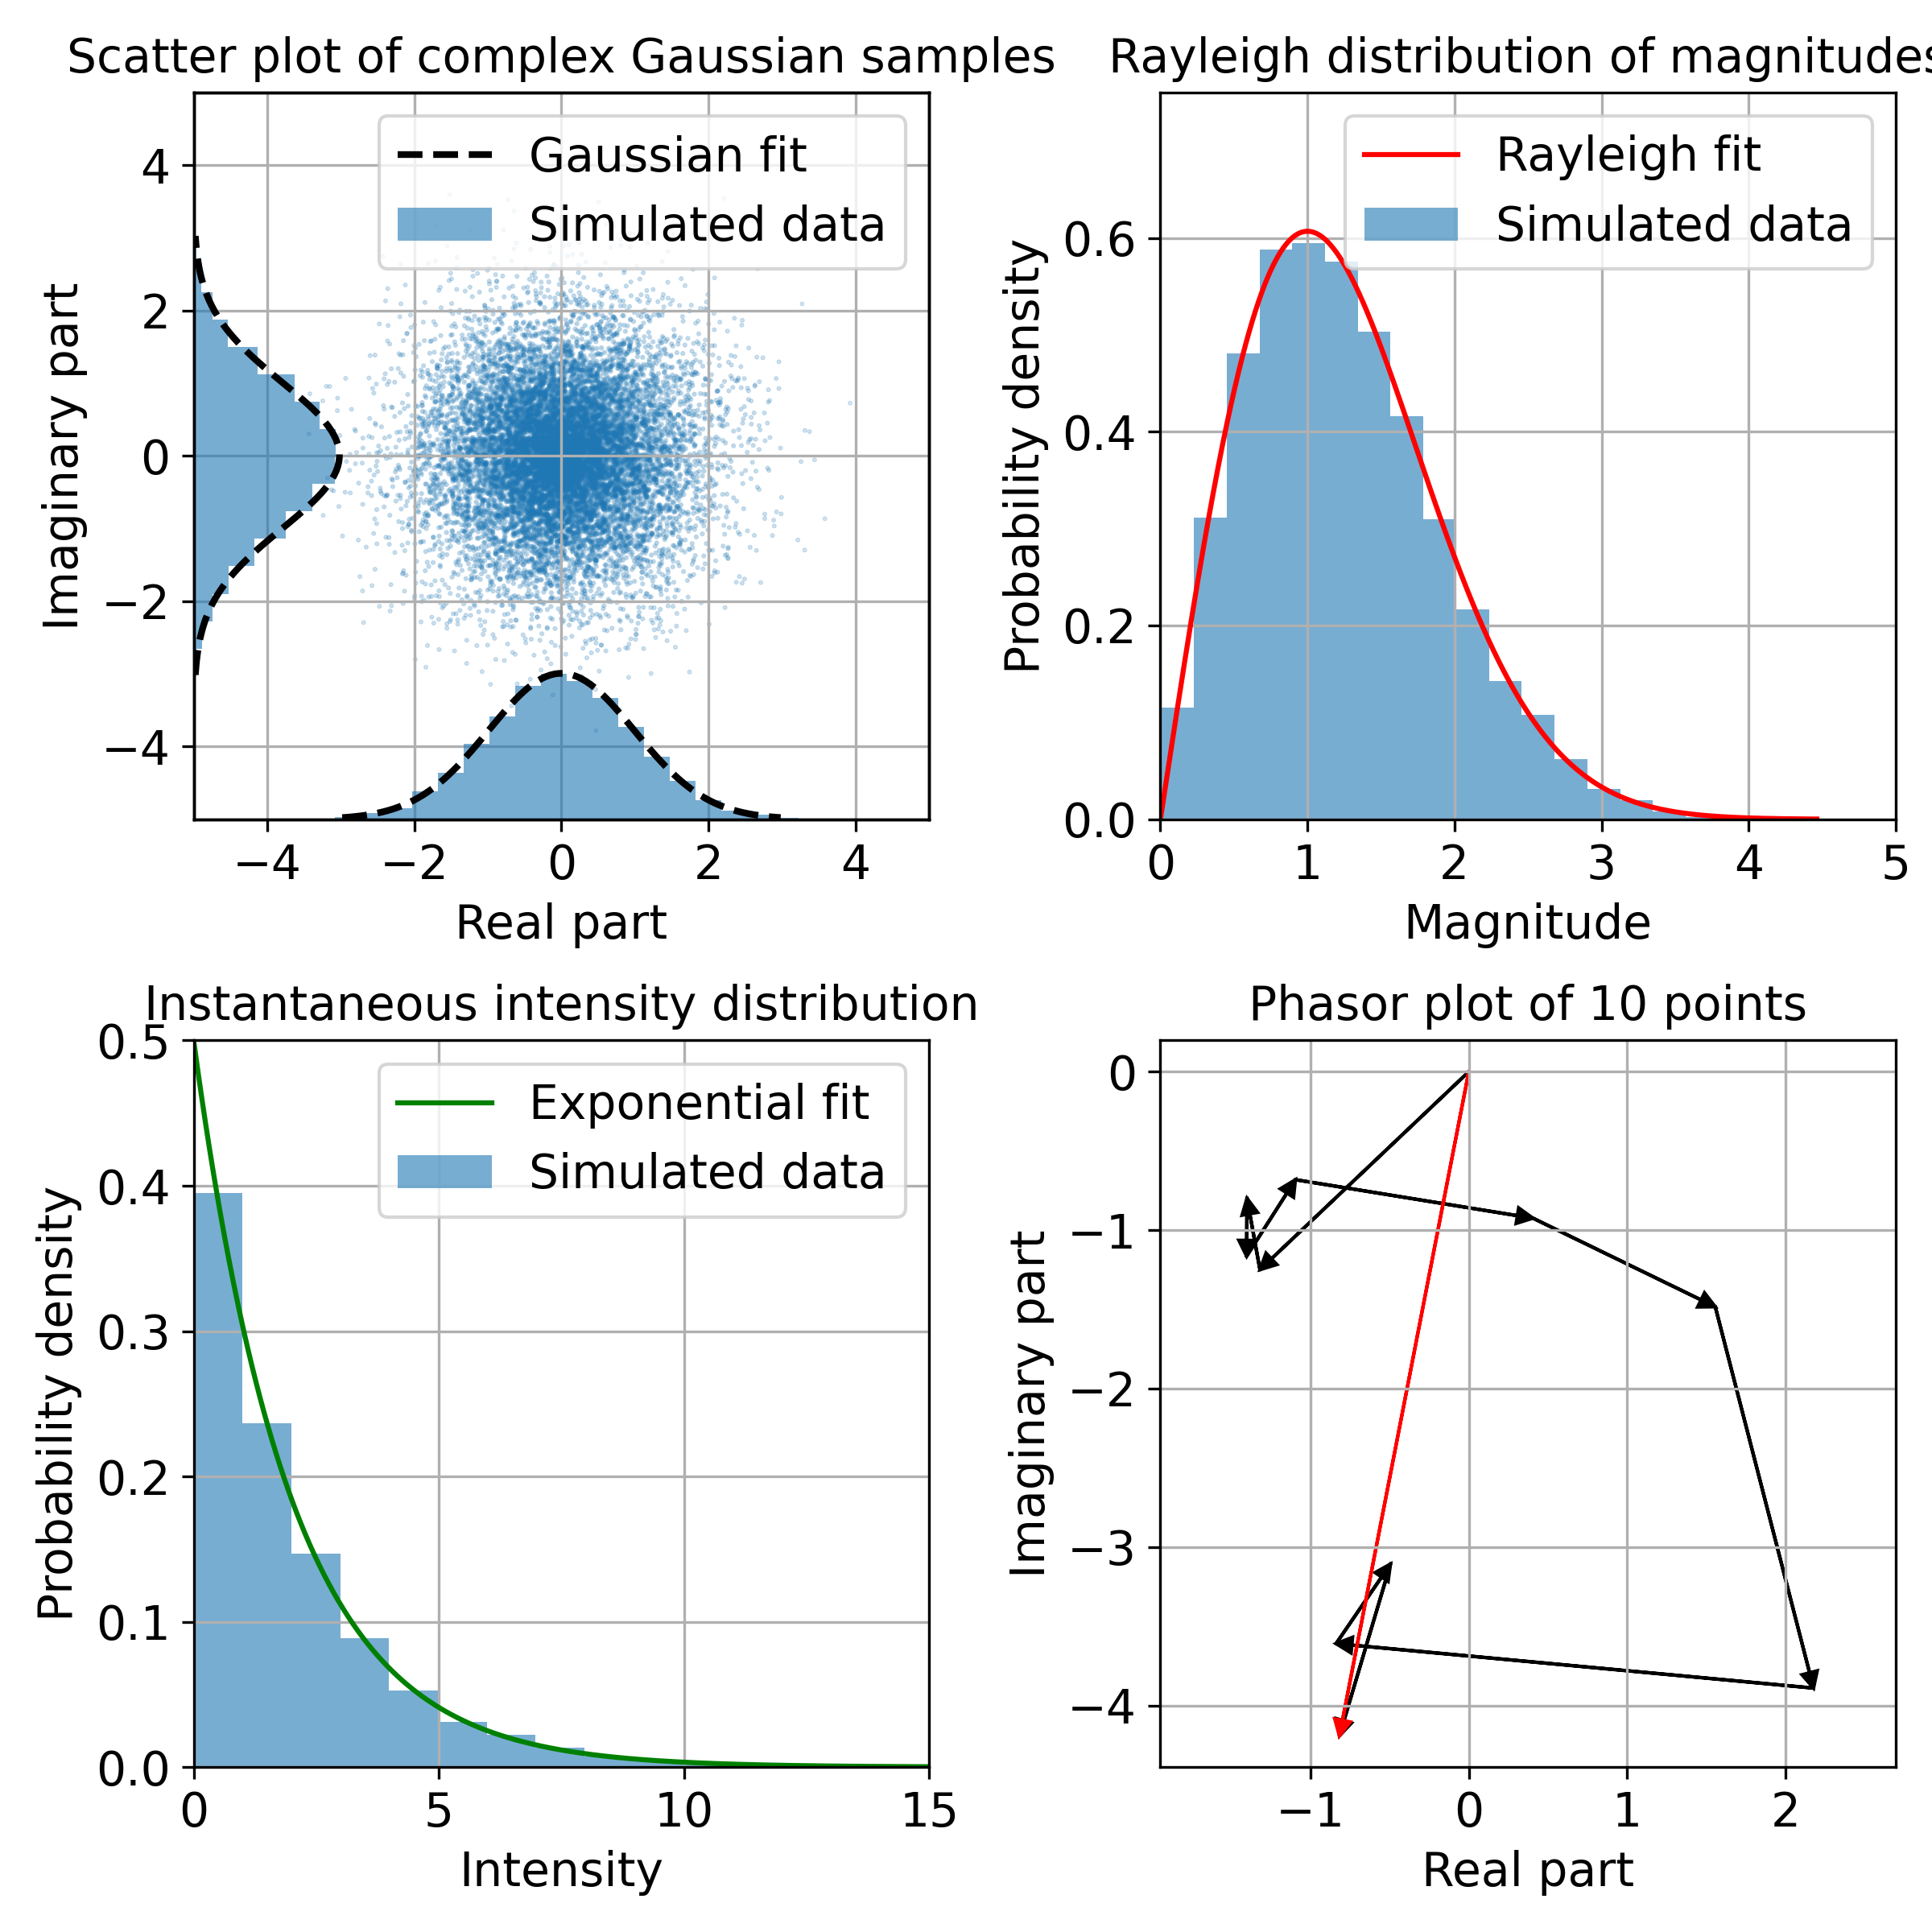
\includegraphics[width=0.75\linewidth]{content/images/Statistical_Optics/gaussian_process.png}
        \captionsetup{justification=centering}
        \caption{Gaussian random process visualisation, dispersion equals unity. Upper left subplot is 10000 samples marked at imaginary plane, upper right subplot Rayleigh distribution, lower left subplot negative exponent distribution, lower right subplot random phasor plotted from ten point.}
        \label{Fig:gaussian_process}
    \end{figure}
    This distribution is called \textit{Rayleigh probability distribution}. In the last equation the dependence on $\phi$ is not presented explicitly that implies that the phase is distributed uniformly for all phase values ($0 \leq \phi \leq 2 \pi$), i.e.:
    \begin{align}
        p(\phi) = \cfrac{1}{\sqrt{2 \pi}}.
    \end{align}
    One can also consider probability density function for the \textit{instantaneous intensity}:
    \begin{align}
        I(t) = A^2(t)
    \end{align}
    and using law for probability functions transformations I obtain:
    \begin{align}
        p(I) = \frac{1}{\langle I \rangle} e^{-I/\langle I \rangle},
    \end{align}
    where $\langle I \rangle = 2 \sigma$. This is distribution is negative exponential distribution. 

    Circular Gaussian random process plays fundamental role for SR and SASE FEL radiation. \rr{make a nice conclusion}
    
\subsection{Quasi-stationary approximation}
    Although may day-to-day sources of radiation can fall under category of stationary or ergodicity non stationary process takes waist majority pivotal role in science. However, it very hard to come up with a generalized theory for this process and derive some practical law. Nevertheless, there is a class of sources that can described in a very similar way as ergodic process that are quasi-stationary sources of radiation. This naming implies that the process is interracial is non-stationary meaning that it starts at some point in time and finishes at another but coherence properties of the radiation resembles ones from ergodic process.
    
    So, if one observes radiation intensity at some point in space and record it over time then the ensemble average will be:
    \begin{align}
        I(t) \coloneqq \langle I(t) \rangle = \lim_{N\to\infty} \frac{1}{N}\sum_{i=1}^{N} E^{[i]}(t)E^{*[i]}(t)
    \end{align}
    Evidently that $I(t)$ is the time envelope of the radiation and obviously depends on time. Then I write the auto-correlation function:
    \begin{align}
        \Gamma(t_1, t_2) = \langle E(t_1)E^*(t_2) \rangle = \lim_{N\to\infty} \frac{1}{N}\sum_{i=1}^{N} E^{[i]}(t_1)E^{*[i]}(t_2)
    \end{align}
    At this point I have not defined anything except for the fact the $I(t) \neq C$ and depends on time, where $C$ is some constant. But let's me introduce normalized version of auto-correlation function $\Gamma(t_1, t_2)$:
    \begin{align}
        g(t_1, t_2) = \frac{\langle E(t_1)E^*(t_2)\rangle}{\sqrt{\langle |E(t_1)|^2\rangle \langle |E^*(t_2)|^2\rangle}} = \frac{\Gamma(t_1, t_2)}{\sqrt{ I(t_1) I(t_2)}}
    \end{align} 
    In a very similar way I can say that $g(t_2, t_1)$ does only depends on time difference $\Delta t = t_2 - t_1$. Having this I obtain:
    \begin{align}
        \Gamma(t_1, t_2) = g(t_2 - t_1) \sqrt{I(t_1) I(t_2)}.
        \label{Eq:Strict_quasi_homo}
    \end{align}
    The radiation sources that have this kind of auto-correlation function I will call quasi-stationary, but there is a "weaker" definition of quasi-homogeneity. If one assumes that the width $g(t_2 - t_1)$ is much smaller at the scale of $I(t)$ then the resulting expression is the following:
    \begin{align}
        \Gamma(t_1, t_2) = g(t_2 - t_1)I\bigg(\frac{t_1 + t_2}{2}\bigg)
        \label{Eq:weak_quasi_homo}
    \end{align}
    This radiation source representation is to some extend similar to quasi-homogeneity in transverse domain~\cite{goodman_statistical_2015}. To my best knowledge there is only few mentions of Eq.~\ref{Eq:weak_quasi_homo}~\cite{lajunen_quasi-stationary_2006, ahad_quasi-monochromatic_2017} in optics community and authors of~\cite{geloni_statistical_2006} resulted in this expression for synchrotron radiation. The results of the paper I will discus later in this thesis.
    
\subsection{Cross-spectral density and generalized Wiener-Khinchin theorem}
    I can calculate auto correlation function in omega domain by definition multiplying Fourier images of the two field  $E(t_1)$ and $E(t_2)$ and taking ensemble average:
    \begin{align}
        \langle \bar{E}(\omega_1)\bar{E}^*(\omega_2) \rangle = \frac{1}{(2 \pi)^2} \iint \limits_{-\infty}^{\infty} \langle E(t_1)E^*(t_2) \rangle e^{i \omega_1 t_1 - \omega_2 t_2} dt_1 dt_2, 
        \label{Eq:cross_spectral_density_dif}
    \end{align}
    in the expression I dragged ensemble averaging under the signs of the integral. Using the expression Eq.~\ref{Eq:weak_quasi_homo} and substituting this in Eq.~\ref{Eq:cross_spectral_density_dif} I obtain:
    \begin{align}
        \langle \bar{E}(\omega_1)\bar{E}^*(\omega_2) \rangle = \frac{1}{(2 \pi)^2} \iint \limits_{-\infty}^{\infty}  g(t_2 - t_1)I\bigg(\frac{t_1 + t_2}{2}\bigg) e^{i \omega_1 t_1 - \omega_2 t_2} dt_1 dt_2, 
    \end{align}
    and now it makes sense to exchange variables $t_1, t_2$ for $\Delta t = t_2 - t_1$ and $\bar{t} = (t_2 + t_1)/2$. The clearly leads to the factorization of the integral:
    \begin{align}
        \langle \bar{E}(\omega_1)\bar{E}^*(\omega_2) \rangle = \frac{1}{(2 \pi)^2} \int \limits_{-\infty}^{\infty}  g(\Delta t) e^{i \bar{\omega} \Delta t} d \Delta t  \int \limits_{-\infty}^{\infty} I(\bar{t}) e^{-i \Delta \omega \bar{t}} d\bar{t} = \bar{I}(\bar{\omega})f_{\omega}(\Delta \omega).
        \label{Eq:general_WKh_t}
    \end{align}
    This result in Eq.~\ref{Eq:general_WKh_t} I will refers as generalized Wiener-Khinchin theorem, although it is difficult to find this result elsewhere except for~\cite{geloni_statistical_2006}. Similar expression can be formulated for stationary radiation where $I(\bar{t})$ turns in constant $C$ and one obtains integral:
    \begin{align}
        \langle \bar{E}(\omega_1)\bar{E}^*(\omega_2) \rangle = \frac{C}{(2 \pi)^2} \int \limits_{-\infty}^{\infty}  g(\Delta t) e^{i \bar{\omega} \Delta t} d \Delta t  \int \limits_{-\infty}^{\infty} e^{-i \Delta \omega \bar{t}} d\bar{t} = \bar{I}(\bar{\omega})\delta(\Delta \omega),
        \label{Eq:WKh_t_derivation}
    \end{align}
    where the latter integral equal delta function: $\delta(\Delta \omega)$ and one can recognise that radiation spectral density or just spectrum is related with auto correlation function via a Fourier transform.
    \begin{align}
        \bar{I}(\bar{\omega}) = \frac{1}{(2 \pi)^2} \int \limits_{-\infty}^{\infty}  g(\Delta t) e^{i \bar{\omega} \Delta t} d \Delta t,
        \label{Eq:WKh_t}
    \end{align}
    Both expression under Eqs.~\ref{Eq:general_WKh_t} and~\ref{Eq:WKh_t} plays essential role in coherence theory on an equal footing with van Cittert-Zernike theorem, which I present in the next section. 

\section{Transverse coherence properties of quasi-stationary sources}
\label{Sec:Transverse coherence properties of quasi-stationary sources}
    Previously, I only considered sources in the time-frequency domain, while real fields exist in three-dimensional space. In this section, I will introduce transverse variables into the autocorrelation function. Then, I will classify the types of sources in terms of the factorizability of the cross-spectral density function in a manner very similar to what I have done for the longitudinal domain. After this, I will provide proof of the van Cittert-Zernike theorem and its generalized version for quasi-homogeneous sources. This chapter will be the last one on the general laws of statistical optics, and it will be followed by practical applications of the theory to synchrotron and free-electron laser radiation.

\subsection{Adding transverse domain}
    In the previous section, the signal was effectively observed through a pinhole. As I consider optical phenomena, not many of them truly occur in the time-frequency domain only -- the signal's propagation direction -- and extend into the transverse domains. Therefore, the expressions I previously provided should be adjusted accordingly to correctly reflect the statistical properties in transverse dimensions.
    Looking at Eq.~\ref{Eq:general_WKh_t}, I assume that $I(\bar{t})$ does not depend on transverse coordinates and I rename this distribution to $f(\bar{t})$. And the all the dependence on transverse variables $\vec{r}_1, \vec{r}_2$ goes to the $g_t$.
    \begin{align}
        \Gamma_{\omega}(\vec{r}_1, \vec{r}_2, \omega_1, \omega_2) = \frac{1}{(2 \pi)^2} \int \limits_{-\infty}^{\infty}  g_t(\vec{r}_1, \vec{r}_2, \Delta t) e^{i \bar{\omega} \Delta t} d \Delta t  \int \limits_{-\infty}^{\infty} f(\bar{t}) e^{-i \Delta \omega \bar{t}} d\bar{t} = G_{\omega}(\vec{r}_1, \vec{r}_2, \bar{\omega})\bar{f}(\Delta \omega),
        \label{Eq:general_WKh_t}
    \end{align}    
    This representation results in the appearance of the cross-spectral density function $G_{\omega}(\vec{r}_1, \vec{r}_2, \bar{\omega})$ in a manner similar to that done for stationary sources, along with the $\bar{f}(\Delta \omega)$ function that describes spectral correlation.  This type of radiation representation, as shown in Eq.~\ref{Eq:general_WKh_t}, adds another level of simplicity but proves to be very useful later.

\subsection{Cross-spectral function distribution at the source}
    In this section I will introduce different definition of  types of the sources describing its transverse coherence properties. Normalized version of the cross-spectral density function has the following form:
    \begin{align}
        g(\vec{r}_1, \vec{r}_2, \omega; 0) = \frac{G(\vec{r}_1, \vec{r}_2, \omega; 0)}{\sqrt{I(\vec{r}_1, \omega; 0)I(\vec{r}_2, \omega; 0)}}.
    \end{align}
    Then one can express cross-spectral density through it and also assume that coherence length is distributed homogeneously across intensity distribution:
    \begin{align}
        G(\vec{r}_1, \vec{r}_2, \omega; 0) =  g(\Delta \vec{r}, \omega; 0){\sqrt{I(\vec{r}_1, \omega)I(\vec{r}_2, \omega; 0)}},
    \end{align}
    which means that the width of $g(\Delta \vec{r}, \omega; 0)$ does not change across the intensity distribution. This kind of radiation source is called quasi-homogeneous~\cite{goodman_statistical_2015}. I can simplify the expression further and make further assumptions on the width of $g(\Delta \vec{r}, \omega; 0)$ function to be much smaller then radiation envelope $I(\bar{\vec{r}}, \omega; 0)$:
    \begin{align}
        G(\vec{r}_1, \vec{r}_2, \omega; 0) =  g(\Delta \vec{r}, \omega; 0)I(\vec{\bar{r}}, \omega).
        \label{Eq:quasi_homogeneous_source_weak}
    \end{align}
    In the limit case of fully incoherent source this degenerate to the following expression:
    \begin{align}
        G(\vec{r}_1, \vec{r}_2, \omega; 0) =  I(\vec{\bar{r}}, \omega; 0)\delta(\Delta \vec{r}),
        \label{Eq:incoherent_source}        
    \end{align}
    where Dirac delta function is introduced. This kind of source describes fully incoherent sources or this kind of sources when one cannot resolve the size of $g(\Delta \vec{r})$
    
\subsection{Propagation law for cross-spectral density function in free space}
    Another essential problem in coherence theory concerns the propagation of coherence properties through an optical system, which includes various optical elements interspaced with free space. By its nature, a single statistical realization of a field from a random process behaves identically to any other radiation field, adhering to the wave equation. Therefore, one effective method to calculate the statistical properties of radiation at the plane $S'$, given a specific distribution at the plane $S$, is to directly apply the corresponding propagator—or a sequence of propagators—through the optical system. Although this approach is practical, it can also be cumbersome to an extent. It necessitates propagating each field sample from $S$ to $S'$ or deriving an analytical expression for the corresponding propagator to apply to the field distribution.
 
    In the simplified scenario of just free space, it is possible to derive a highly useful law describing how the cross-spectral density function or the mutual coherence function evolves. This case is particularly practical because there is typically some free space between the radiation source and the entrance of an optical system. Understanding the coherence properties of radiation just before it enters the optical system is valuable. Therefore, let me begin by examining the wave equation directly in free space:
    \begin{align}
        \nabla^2_1 \vec{E}(\vec{r}_1, t_1) - \cfrac{1}{c^2} \frac{\partial^2 \vec{E}(\vec{r}_1, t_1)}{\partial t_1^2} = 0
        \label{Eq:wave_eq}
    \end{align}
    By multiplying this with $\vec{E}^(\vec{r}_2, t_2)$, where $^*$ denotes the complex conjugate, and then incorporating it under the differentiation signs:
    \begin{align}
        \nabla^2_1 \big[\vec{E}(\vec{r}_1, t_1) \vec{E}(\vec{r}_2, t_2)\big]- \cfrac{1}{c^2} \frac{\partial^2 \big[\vec{E}(\vec{r}_1, t_1) \vec{E}(\vec{r}_2, t_2)\big]}{\partial t_1^2} = 0.
    \end{align}
    By ensemble averaging this equation, and noting that the averaging operation can be interchanged with differentiation, I obtain:
    \begin{align}
        \nabla^2_1 \Gamma(\vec{r}_1, \vec{r}_2, t_1, t_2)  - \cfrac{1}{c^2} \frac{\partial^2 \Gamma(\vec{r}_1, \vec{r}_2, t_1, t_2)}{\partial t_1^2} = 0,
    \end{align}
    To close this differential system, one can derive the complementary equation in the same manner:
    \begin{align}
        \nabla^2_2 \Gamma(\vec{r}_1, \vec{r}_2, t_1, t_2)  - \cfrac{1}{c^2} \frac{\partial^2 \Gamma(\vec{r}_1, \vec{r}_2, t_1, t_2)}{\partial t_2^2} = 0,
    \end{align}
    By taking the Fourier transform of both sides in the time domain, I obtain a system for the cross-spectral density function $G(\vec{r}_1, \vec{r}_2, \omega)$ that follows:
    \begin{align}
        \nabla^2_1 G(\vec{r}_1, \vec{r}_2, \omega) + k^2 G(\vec{r}_1, \vec{r}_2, \omega) = 0\\
        \nabla^2_2 G(\vec{r}_1, \vec{r}_2, \omega) + k^2 G(\vec{r}_1, \vec{r}_2, \omega) =0 .
    \end{align}
    where I divided each equation by $f(\Delta \bar{\omega})$. This system of two Helmholtz equations have a known solution. Assuming that we know the distribution $G(\vec{r}'_1, \vec{r}'_2, \omega)$ in the $S$ plane, where $z=0$, we can solve this system using the Green's function for the Helmholtz equation with Dirichlet boundary conditions. This approach allows us to derive the following law for propagating the cross-spectral density function:
    \begin{align}
        G(\vec{r}_1, \vec{r}_2, \omega) = \bigg(\cfrac{k}{ 2 \pi} \bigg)^2 \iint_{z=0} G(\vec{r}'_1, \vec{r}'_2, \omega) \cfrac{e^{i k (R_2 - R_1)}}{R_1 R_2} \cos(\theta_1) \cos(\theta_2) d^2r'_1 d^2r'_2
        \label{Eq:G_propagation_law}
    \end{align}
    \begin{wrapfigure}{r}{0.5\textwidth}
        \centering
        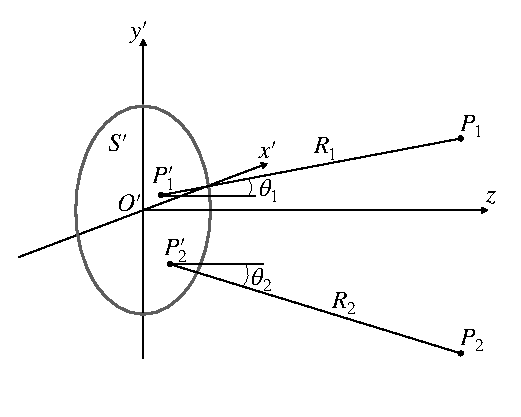
\includegraphics[width=0.95\linewidth]{content/images/Statistical_Optics/coh_prop_scheme.pdf}
        \captionsetup{justification=centering}
        \caption{Geometry of the cross-spectral density propagation in the free-space. Adapted from~\rr{cite}}
        \label{Fig:coh_prop_scheme}
    \end{wrapfigure}
    This expression is foundational for deriving the van Cittert-Zernike theorem, which I will discuss in the next section. Historically, the van Cittert-Zernike theorem was formulated using Huygens' principle, resulting in an expression for the mutual intensity function~\cite{van_cittert_wahrscheinliche_1934, zernike_concept_1938}.
    Interestingly, it should be noted that the cross-spectral density obeys the same laws as the mutual intensity function $J(\vec{r}_1, \vec{r}_2) = g_t(\vec{r}_1, \vec{r}_2, \Delta =~0)$,~\cite{goodman_statistical_2015, mandel_wolf}. It is important to remember that this holds true only for quasi-monochromatic sources. Therefore, I will continue to present the results for the theorem using the cross-spectral density.

\subsubsection{The van Cittert-Zernike theorem}
    Equation~\ref{Eq:G_propagation_law} is highly general and can be applied to any propagating field to calculate its cross-spectral distribution upon propagation. However, this integral can be further simplified to derive practical formulas for specific types of sources—namely, fully incoherent and partially coherent sources under the quasi-homogeneous approximation -- these relation constitutes van Cittert-Zernike theorem and its generalised version. 
    
    Assuming the paraxial approximation, I can write the following expression for the mutual intensity function derived from Equation~\ref{Eq:G_propagation_law}:
    \begin{align}
        G(\vec{r}_1, \vec{r}_2, \omega) = \bigg(\cfrac{k}{ 2 \pi} \bigg)^2 \iint_{\mathcal{S}} G(\vec{r}'_1, \vec{r}'_2, \omega) \cfrac{e^{i k (R_2 - R_1)}}{R_1 R_2}d^2r'_1 d^2r'_2
        \label{Eq:G_propagation_law_4_VCZ}
    \end{align}
    \begin{figure}[h!]
        \centering
        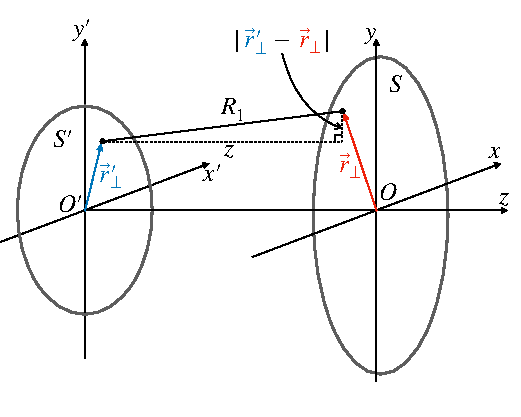
\includegraphics[width=0.5\linewidth]{content/images/Statistical_Optics/coh_prop_scheme_2.pdf}
        \captionsetup{justification=centering}
        \caption{Geometry of the cross-spectral density propagation in the free-space. Adapted from~\rr{cite}.}
        \label{Fig:coh_prop_scheme_2}
    \end{figure}
    If the cross-spectral density function is observed in the far zone Eq.~\ref{Eq:G_propagation_law_4_VCZ} can be further simplified using the relations:
    \begin{align}
        \begin{array}{c}
            R_{1, 2}\approx  z + \cfrac{|\vec{r}'_{1, 2{\perp}} - \vec{r}_{1, 2{\perp}}|^2}{2z}\\
            \\
            R_{1}R_{1} \approx z^2
        \end{array}
        \label{Eq:R1R2_simp}
    \end{align}
    for simplicity of the notation it make sense to redefine $\vec{r}_{1, 2} :=\vec{r}_{1, 2{\perp}}$ and the same for $\vec{r}'_{1, 2} :=\vec{r}'_{1, 2{\perp}}$ (but only for till the end of the current Section~\ref{Sec:Statistical optics for quasi-homogeneous sources}).

    Now I would like to simplify $R_2 - R_1$ in the exponent. Using first relation in Eq.~\ref{Eq:R1R2_simp}:
    \begin{align}
        R_2 - R_1 = \cfrac{1}{2z} \bigg(|\vec{r}_{2}|^2 - 2|\vec{r}_{2} \cdot \vec{r}'_{2}| + |\vec{r}'_{2}|^2 - |\vec{r}_{1}|^2 + 2|\vec{r}_{1} \cdot \vec{r}'_{1}| - |\vec{r}'_{1}|^2\bigg)
    \end{align} 
    and introducing new variables $\vec{\bar{r}} = \vec{r}_1 - \vec{r}_2$ and $\Delta\vec{r} = (\vec{r}_2 + \vec{r}_1)/2$ and the same for the primed set of variables, this leads me to: 
    \begin{align}
        \begin{array}{c}
        |\vec{r}_{2}|^2 - |\vec{r}_{1}|^2 = -2\vec{\bar{r}}\cdot\Delta\vec{r} \\
        |\vec{r}'_{2}|^2 - |\vec{r}'_{1}|^2 = -2\vec{\bar{r}}'\cdot\Delta\vec{r}' \\
        |\vec{r}_{1} \cdot \vec{r}'_{1}| - |\vec{r}_{2} \cdot \vec{r}'_{2}| = \vec{\bar{r}}\cdot\Delta\vec{r}' + \vec{\bar{r}}'\cdot\Delta\vec{r},
        \end{array}
    \end{align}
    where $\cdot$ denotes scalar product. Then I substitute this in Eq.~\ref{Eq:G_propagation_law_4_VCZ} and obtain:
    \begin{align}
        G(\vec{\bar{r}}, \Delta\vec{r}, \omega; 0) = \bigg(\cfrac{k}{ 2 \pi} \bigg)^2 \cfrac{e^{-\frac{i k}{z} \vec{\bar{r}}\cdot\Delta\vec{r}}}{z^2}     \iint_{\mathcal{S}} G(\vec{\bar{r}}', \Delta\vec{r}', \omega, z) e^{\frac{i k}{z} (\vec{\bar{r}}\cdot\Delta\vec{r}' + \Delta\vec{r}\cdot\vec{\bar{r}}')} d\vec{\bar{r}}' d\Delta\vec{r}' 
        \label{Eq:VCZ_general_form}
    \end{align}
    Here, I neglected the term $2\vec{\bar{r}}'\cdot\Delta\vec{r}'$ in the exponent under assumption condition $\vec{\bar{r}}'\cdot\Delta\vec{r}'/ (\lambda z) \ll 1$, which basically can be interpreted as placing the observation plane ($S'$) in far zone.
    
    Using this definition of fully incoherent source and substituting this in Eq.~\ref{Eq:VCZ_general_form} I obtains:
    \begin{align}
        G(\vec{\bar{r}}, \Delta\vec{r}, \omega; z) &= \cfrac{e^{- i \frac{k}{z} \vec{\bar{r}}\cdot\Delta\vec{r}}}{(\lambda z)^2} \iint_{\mathcal{S}} I(\vec{\bar{r}}', \omega)\delta(\Delta \vec{r}') e^{i \frac{k}{z} (\vec{\bar{r}}\cdot\Delta\vec{r}' + \vec{\bar{r}}'\cdot\Delta\vec{r})} d\vec{\bar{r}}' d\Delta\vec{r}' \nonumber = \\
        &\fcolorbox{black}{yellow!30}{\rule[-4ex]{0pt}{10ex}$\displaystyle \stackrel{\text{van Cittert-Zernike theorem}}{\cfrac{e^{-i \frac{k}{z} \vec{\bar{r}}\cdot\Delta\vec{r}}}{(\lambda z)^2} \int_{\mathcal{S}} I(\vec{\bar{r}}', \omega) e^{i \frac{k}{z} \vec{\bar{r}}'\cdot\Delta\vec{r}} d\vec{\bar{r}}'}$}
        \label{Eq:VCZ_incoherent}
    \end{align}
    This is the original result of the van Cittert-Zernike theorem but the theorem can be extended for the more general source representation under Eq.~\ref{Eq:quasi_homogeneous_source_weak}. Again using integral in Eq.~\ref{Eq:VCZ_general_form} and substituting in it the expression from Eq.~\ref{Eq:quasi_homogeneous_source_weak} I obtain:
    \begin{align}
        G(\vec{\bar{r}}, \Delta\vec{r}, \omega; z) &=  \cfrac{e^{-i \frac{k}{z} \vec{\bar{r}}\cdot\Delta\vec{r}}}{(\lambda z)^2} \iint_{\mathcal{S}} g(\Delta \vec{r}', \omega; 0)I(\vec{\bar{r}}', \omega) e^{i \frac{k}{z} (\vec{\bar{r}}\cdot\Delta\vec{r}' + \vec{\bar{r}}'\cdot\Delta\vec{r})} \, d\vec{\bar{r}}' \, d\Delta\vec{r}' \nonumber =\\
        &\fcolorbox{black}{yellow!30}{\rule[-4ex]{0pt}{10ex}$\displaystyle \stackrel{\text{generalised van Cittert-Zernike theorem}}{\cfrac{e^{-i \frac{k}{z} \vec{\bar{r}}\cdot\Delta\vec{r}}}{(\lambda z)^2} \int_{\mathcal{S}} g(\Delta \vec{r}', \omega; 0) e^{-i \frac{k}{z} \vec{\bar{r}}\cdot\Delta\vec{r}'} \, d\Delta\vec{r}'  \int_{\mathcal{S}} I(\vec{\bar{r}}', \omega) e^{i \frac{k}{z} \vec{\bar{r}}'\cdot\Delta\vec{r}} \, d\vec{\bar{r}}'}$}
        \label{Eq:VCZ_partially_coherent}
    \end{align}
    \begin{figure*}[h!]
      \centering
      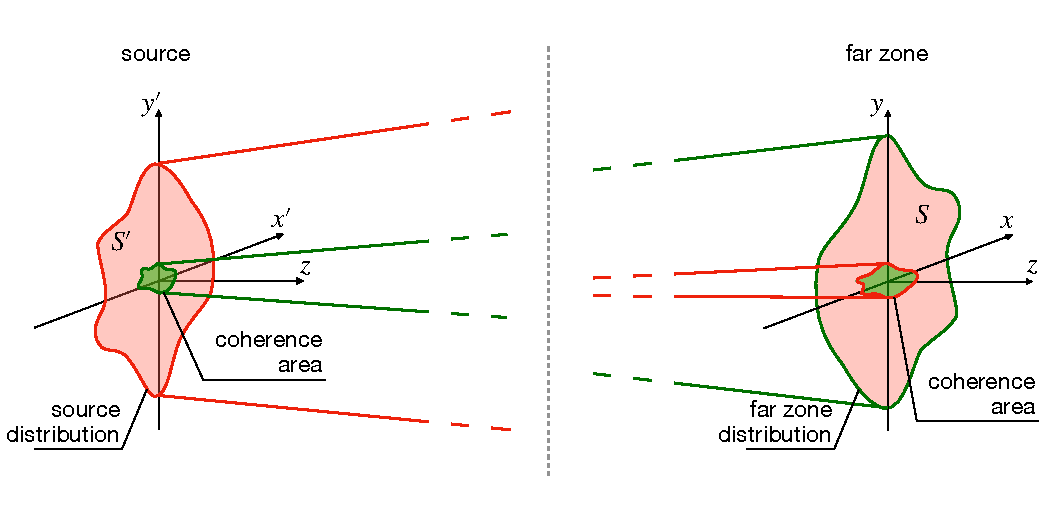
\includegraphics[width=0.95\linewidth]{content/images/Statistical_Optics/VCZ_scheme.pdf}
      \captionsetup{justification=centering}
      \caption{Visual representation of the generalised van Cittert-Zernike theorem. }
      \label{Fig:coh_prop_scheme}
    \end{figure*}
    This is a result for a partially coherent source with cross-spectral density distribution as in given in Eq.~\ref{Eq:quasi_homogeneous_source_weak}. The theorem provide one with a relation of the intensity and cross-spectral distributions at the source and in the far zone. Surely, it is easy to show that the inverse version of the van Cittert-Zernike theorem holds as well. So, I present all the relation in the diagram in Fig.~\ref{Fig:VCZ_scheme}.
    \begin{figure}[h!]
        \centering
        \begin{tikzpicture}[
            % Define styles
            node distance=2cm,
            mynode/.style={
              shape=ellipse,
              draw,
              text width=2.5cm,
              align=center
            },
            bluearrow/.style={
              <->,
              >=latex,
              blue,
              thick
            },
            redarrow/.style={
              <->,
              >=latex,
              red,
              thick
            },
            bluetext/.style={
              text=blue
            },
            redtext/.style={
              text=red
            }
          ]
        
          % Nodes
          \node[mynode] (g0) {$g(\Delta\mathbf{\hat{r}}; \mathbf{0})$};
          \node[mynode, right=of g0] (I0) {$I(\mathbf{\hat{r}}; \mathbf{0})$};
          \node[mynode, below=of g0] (gz) {$\dfrac{g( \Delta\mathbf{\hat{\theta}}; \mathbf{\hat{z}})}{\exp[i\mathbf{\hat{z}} \Delta\mathbf{\hat{\theta}} \cdot \mathbf{\theta}]}$};
          \node[mynode, right=of gz] (Iz) {$I(\mathbf{\hat{\theta}}; \mathbf{\hat{z}})$};
        
          % Arrows with FT labels
          \draw[bluearrow] (g0) -- (Iz) node[pos=0.25, above, bluetext] {FT};
          \draw[redarrow] (gz) -- (I0) node[pos=0.75, above, redtext] {FT};
        \end{tikzpicture}
        \caption{Relations between intensity and cross-spectral distributions at the source and in the far zone that van Cittert-Zernike theorem and its inverse version set.}
        \label{Fig:VCZ_scheme}
    \end{figure}
    The van Cittert-Zernike theorem (and its generalised version) provide on with very practical relation between the source size and the observed coherence spot in the far zone and forms the basis for coherence theory for studying synchrotron radiation sources. 

\section{Simulations of the partially coherent sources}   
    Numerical modeling of the stochastic sources is thought process that may require a lot of numerical resources. Considering the task from a more general point of view one need to solve stochastic partial differential equation,    where right hand side of the equation depends on random variables:
    \begin{align}
        c^2 \nabla^2 \vec{E} - \frac{\partial^2 \vec{E}}{\partial t^2} = - 4 \pi c^2 \vec{\nabla} (-e) \sum_{i=1}^{N_e}\delta(\vec{r} - \vec{r}_i'(t)) + 4 \pi (-e) \sum_{i=1}^{N_e}\frac{\partial (\vec{v}_i(t)\delta(\vec{r} - \vec{r}_i'(t)))}{\partial t},
    \end{align}
    where particles are distributed according the phase space of the electron beam. Moreover, this problem must be solved $N_b$ times according to the required number of statistical realizations each time for unique random distribution of the of the electrons within the phase space.
    This problem can be simplified if one make use of superposition law of the electrodynamics and solve this equation for a single electron, what I have done in the Chapter \rr{2} and then sum up all the contributions, but the problem scales up, as for the obtaining real field the equation should be solved $N_e$-times and then one need to collect $N_b$ realizations, this would be the most general approach and, if it is possible to say this way, straightforward for solving this problem.

    \rr{write about micro electrons}
    
    Obviously, such a direct approach is not always required or even feasible. As we have discussed in the previous section, the task of describing coherent properties of x-ray synchrotron radiation boils down to summing up \oo{mutual intensity contribution} from separate electrons due to poor longitudinal coherence. As you can see this requires solving solution single electron equation $N_e$ times.

    The main problem in such simulation is not only simulate a radiation but also propagate it through an optical system. One approach is to simulated the stochastic field according: sum up all contribution from all electrons and then create a hole ensemble of these fields. Another approach is to propagate radiation from all electrons separately and sum up their mutual intensity at the point of interest along a optical line, the third approach is to decompose the known field on the coherent modes and propagate these modes. The approach that provide the most physics simulation is propagation of the stochastic field itself. \oo{discuss why?}

    While modeling the whole stochastic field is not a trivial task, as I have shown the straightforward approach requires calculation from $N_eN_b$ electrons. But is knowledge of single electron radiation is really required as soon as one knows the exact intensity distribution and the cross spectral density function according to Eq.~\ref{}? 

\section{Coherence properties of X-ray emission of synchrotron radiation source}
In this chapter we at first present some reasoning on the synchrotron radiation statistical properties in time domain to follow usual reasoning of statistical optics. But then switch to omega domain. With this I hope, it will be very demonstrative to show the link between statistical optics written mostly for stationary sources and statistical properties of SR and SASE FEL radiation.
    
    In the section I will talk about intrinsic properties of synchrotron radiation. For FEL SASE the same reasoning can be applied, as radiation starts as usual synchrotron radiation and then being exponentially amplified due to radiation with electron beam interaction, which is effectively acts on radiation as a linear \rr{filter} \oo{it's not a filter but transform}. Synchrotron radiation originates from ultra relativistic electron beams that is restricted in time domain. Hence, naturally emitted radiation is also restricted in time, which in principal mean that that kind of bursts of radiation is non-stationarity. For synchrotron radiation it is very natural to define a realisation as radiation pulse from an electron beam passing through a magnetic structure and observed by an experimentation located at $R$ with respect to some reference frame. It is very important to note that each realization is unique in any case, electrons are distributed randomly within the beam phase space and for each electron beam this distribution is unique. Moreover, if one consider a storage rind with a single one stored electron beam at each tern this distribution will be unique as well, constant shake-the-dice process happens as the electron beam passes through the magnetic structure\footnote{Vacuum tube and the other lattice component are also contribute to the process.} of the storage ring. This process is called \rr{really how?}. 
    
    Thus, an experimentation should only has some trigger to know when the process starts and finishes and then overlay all collected realizations. This last statement we will discuss further on \rr{where?} in this thesis as this "overlay" happens not in time domain but in frequency domain.
    
    Synchrotron radiation is intrinsically a Gaussian process, this fact is easy to show. Distribution of random shift follows \oo{distribution} but as soon as we deal with large number of particles overall contribution will follow Gaussian statistics according the central limit theorem. As the process is Gaussian we can utilize the useful property that every higher order autocorrelation function can be expressed with the second order correlation function.

    In this section I would like to show that x-ray synchrotron radiation follows the theory I have derived in the previous section.
    
    The field from the whole electron beam can be written in the following as the sum from individual electrons:
    \begin{align}
        E_b(z, \vec{r}, t) = \sum_{k=1}^{N_e} E(\vec{\eta}_k, \vec{l}_k, z, \vec{r}, t - t_k), 
    \end{align}
    where $\vec{\eta}_k$ is an electron deflection, $\vec{l}_k$ its off-set and $t_k$ - arrival time with respect to some reference time. It is more practical to consider this field in $\omega$ domain as exactly this kind of field is possible to measure. 
    \begin{align}
        \bar{E}_b(z, \vec{r}, \omega) = \sum_{k=1}^{N_e} \bar{E}(\vec{\eta}_k, \vec{l}_k, z, \vec{r}, \omega)e^{i \omega t_k}, 
        \label{Eq:ebeam_rad_omega}
    \end{align}   
    I would like to study coherence properties of this radiation, so I write \rr{correlation function?}
    \begin{align}
        \Gamma_\omega (z, \vec{r}_1, \vec{r}_2, \omega_1, \omega_2) = \langle \bar{E}_b(z, \vec{r}_1, \omega_1) \bar{E}^*_b(z, \vec{r}_1, \omega_1) \rangle
        \label{Eq:Gamma_omega}
    \end{align} 
    Substituting Eq.~\ref{Eq:ebeam_rad_omega} in Eq.~\ref{Eq:Gamma_omega} I obtain:
    \begin{align}
        \Gamma_\omega (z, \vec{r}_1, \vec{r}_2, \omega_1, \omega_2) = \bigg\langle 
        \sum_{m,n=1}^{N_e} \bar{E}(\vec{\eta}_m, \vec{l}_m, z, \vec{r}, \omega_1)\bar{E}^*(\vec{\eta}_n, \vec{l}_n, z, \vec{r}, \omega_2)e^{i (\omega_1 t_m - \omega_2 t_n)}
        \bigg\rangle
    \end{align}
    and separating sum over the same indexes and over different ones I obtain:
    \begin{align}
        \Gamma_\omega (z, \vec{r}_1, \vec{r}_2, \omega_1, \omega_2) =  
        \sum_{m = 1}^{N_e} \langle\bar{E}(\vec{\eta}_m, \vec{l}_m, z, \vec{r}, \omega_1)\bar{E}^*(\vec{\eta}_m, \vec{l}_m, z, \vec{r}, \omega_2)e^{i (\omega_1 -\omega_2) t_m)}\rangle + \cr
        \sum_{m \neq n}^{N_e} \langle\bar{E}(\vec{\eta}_m, \vec{l}_m, z, \vec{r}, \omega_1)\bar{E}^*(\vec{\eta}_n, \vec{l}_n, z, \vec{r}, \omega_2)e^{i (\omega_1 t_m - \omega_2 t_n)}\rangle.
        \label{Eq:Two_sums}
    \end{align}
    \rr{fantastically} I one may notice that ensemble average $\langle e^{i \omega t_k}\rangle = \int\limits_{-\infty}^{\infty} f(t_k) e^{i \omega t_k} = \bar{f} (\omega)$ according to the definition of the statistical realization in Eq.~\ref{Eq:ensemble_int_avr}. So, I can rewrite Eq.~\ref{Eq:Two_sums} as the following
    \begin{align}
        \Gamma_\omega (z, \vec{r}_1, \vec{r}_2, \omega_1, \omega_2) =  
        \sum_{m = 1}^{N_e} \langle\bar{E}(\vec{\eta}_m, \vec{l}_m, z, \vec{r}, \omega_1)\bar{E}^*(\vec{\eta}_m, \vec{l}_m, z, \vec{r}, \omega_2) \rangle\bar{f}(\omega_1 - \omega_2) + \cr
        \sum_{m \neq n}^{N_e} \langle\bar{E}(\vec{\eta}_m, \vec{l}_m, z, \vec{r}, \omega_1)\bar{E}^*(\vec{\eta}_n, \vec{l}_n, z, \vec{r}, \omega_2)\rangle\bar{f}(\omega_1)\bar{f}(-\omega_2).
        \label{Eq:Two_sums}
    \end{align}
    In the case of x-ray radiation the second term corresponds to the "interference" term between radiation from different electrons. But as the function $\bar{f}(\omega)$ has the width that is inversely proportional to the electron beam duration, so $\bar{f}(\omega_1)\bar{f}(-\omega_2)$ goes to zero very rapidly. Minus sign is very essential here and has very physics meaning here: there is not way that the synchrotron radiation will be amplified unless $\omega\sigma_{\tau} \sim 1$.
    Now we obtain:
    \begin{align}
        \Gamma_\omega (z, \vec{r}_1, \vec{r}_2, \omega_1, \omega_2) =  
        \sum_{m = 1}^{N_e} \langle\bar{E}(\vec{\eta}_m, \vec{l}_m, z, \vec{r}, \omega_1)\bar{E}^*(\vec{\eta}_m, \vec{l}_m, z, \vec{r}, \omega_2) \rangle\bar{f}(\omega_1 - \omega_2) = \cr 
        N_e\langle\bar{E}(\vec{\eta}, \vec{l}, z, \vec{r}, \omega_1)\bar{E}^*(\vec{\eta}, \vec{l}, z, \vec{r}, \omega_2) \rangle\bar{f}(\omega_1 - \omega_2),
        \label{Eq:}
    \end{align}
    where in the last equality I used that fact the result under ensemble averaging is constant distribution and does not depend on chosen electrons.
    One can notice that equivalent definition of ensemble averaging again and transform this averaging in just some over different electrons:
    \begin{align}
        \Gamma_\omega (z, \vec{r}_1, \vec{r}_2, \omega_1, \omega_2) = 
        N_e\langle\bar{E}(\vec{\eta}, \vec{l}, z, \vec{r}, \omega_1)\bar{E}^*(\vec{\eta}, \vec{l}, z, \vec{r}, \omega_2) \rangle\bar{f}(\omega_1 - \omega_2) \cr = 
        N_e \bar{f}(\omega_1 - \omega_2) \sum_{i = 1}^{N_e}\bar{E}(\vec{\eta}_i, \vec{l}_i, z, \vec{r}, \omega_1)\bar{E}^*(\vec{\eta}_i, \vec{l}_i, z, \vec{r}, \omega_2) \textup{or} \cr
        N_e \bar{f}(\omega_1 - \omega_2) \iint \limits_{-\infty}^{\infty}f_{l}(\vec{l}) f_{\eta}(\vec{\eta}) \bar{E}(\vec{\eta}, \vec{l}, z, \vec{r}, \omega_1)\bar{E}^*(\vec{\eta}, \vec{l}, z, \vec{r}, \omega_2)d\vec{l} d\vec{\eta}
        \label{Eq:}
    \end{align}    
    We can see here that calculating $\Gamma_\omega (z, \vec{r}_1, \vec{r}_2, \omega_1, \omega_2)$ only requires knowledge of the electron beam phase space distribution. 

    \rr{write a whole paragraph describing why we can say that $\omega_1 \approx \omega_2$ in the field dependence}
    
    It is useful to introduce cross-spectral density function
    \begin{align}
        G(z, \vec{r}_1, \vec{r}_2, \omega) = \langle\bar{E}(\vec{\eta}, \vec{l}, z, \vec{r}, \omega)\bar{E}^*(\vec{\eta}, \vec{l}, z, \vec{r}, \omega)
    \end{align}
    More often then not radiation is seen through an monochromator with transfer function $T(\omega)$, so one need to rewrite the Eq.~\ref{} as the following: 
    \begin{align}
        \Gamma_\omega (z, \vec{r}_1, \vec{r}_2, \omega_1, \omega_2) = N_e \bar{f}(\omega_1 - \omega_2) G(z, \vec{r}_1, \vec{r}_2, \omega_1) T(\omega_1) T(\omega_2)
    \end{align}

    \subsection{\rr{conformation} of the Wiener–Khinchin theorem for synchrotron radiation}
    \begin{align}
        \Gamma_t(z, \vec{r}_1, \vec{r}_2, t_1, t_2) = 
        \frac{1}{(2 \pi)^2}\iint \limits_{-\infty}^{\infty} \Gamma_\omega (z, \vec{r}_1, \vec{r}_2, \omega_1, \omega_2) e^{-i\omega_1 t_1} e^{i\omega_2 t_2} d\omega_1 d\omega_2 = \cr
        \frac{N_e}{(2 \pi)^2}\iint \limits_{-\infty}^{\infty} \bar{f}(\omega_1 - \omega_2) G(z, \vec{r}_1, \vec{r}_2, \omega_1) T(\omega_1) T(\omega_2) e^{-i\omega_1 t_1} e^{i\omega_2 t_2} d\omega_1 d\omega_2
    \end{align}
    \rr{doing all assumptions}

    \begin{align}
        \Gamma_t(z, \vec{r}_1, \vec{r}_2, t_1, t_2) = 
        \frac{N_e}{(2 \pi)^2}\int \limits_{-\infty}^{\infty} \bar{f}(\Delta \omega) e^{-i\Delta \omega \bar{t}}d\Delta \omega \int \limits_{-\infty}^{\infty} G(z, \vec{r}_1, \vec{r}_2,\bar{\omega}) T(\bar{\omega}) e^{i\bar{\omega} \Delta t}d\bar{\omega}
    \end{align}
    One can see that this result is an reoccurrence of generalized Wiener-Khinchin theorem~\ref{Eq:general_WKh_t} but source specific.


    \subsection{Heuristic approach: homogeneous/stationary source}
    \label{sec:Heuristic approach: homogeneous/stationary source}
        I will try to build a fully incoherent field as the following:
        \begin{align}
            \phi(\vec{r}) = \sqrt{I(\vec{r})} \mathcal{N}(\vec{r}),
        \end{align}
        where $\langle \mathcal{N}(\vec{r}_1)\mathcal{N}(\vec{r}_2)\rangle = \delta(\vec{r}_2 - \vec{r}_1)$. It easy to find that:
        \begin{align}
            \langle \phi(\vec{r})\phi^*(\vec{r}) \rangle = I(\vec{r}),
        \end{align}        
        Calculating
        \begin{align}
            \langle \phi(\vec{r}_1)\phi^*(\vec{r}_2) \rangle = \sqrt{I(\vec{r}_1)I(\vec{r}_2)} \langle \delta(\vec{r}_2 - \vec{r}_1) \rangle,
        \end{align}          
        And the same it can be shown that the inverse space representation of the field:
        \begin{align}
            \bar{\phi}(\vec{k}) = \int \limits_{-\infty}^{\infty} \sqrt{I(\vec{r})} \mathcal{N}(\vec{r}) e^{i \vec{r}\vec{k}}d\vec{r}
        \end{align}


        \begin{align}
            \langle \bar{\phi}(\vec{k}_1) \bar{\phi}(\vec{k}_2) \rangle = \bigg \langle \iint \limits_{-\infty}^{\infty}  \sqrt{I(\vec{r}_1)I(\vec{r}_1)} \mathcal{N}(\vec{r}_1)\mathcal{N}(\vec{r}_2) e^{i (\vec{r}_1\vec{k}_1 - \vec{r}_2\vec{k}_2)}d\vec{r}_1d\vec{r}_2 \bigg \rangle = \cr
            =\iint \limits_{-\infty}^{\infty} \sqrt{I(\vec{r}_1)I(\vec{r}_1)} \delta(\vec{r}_1 - \vec{r}_2) e^{i (\vec{r}_1\vec{k}_1 - \vec{r}_2\vec{k}_2)}d\vec{r}_1d\vec{r}_2.
        \end{align}

        \begin{align}
            \langle \bar{\phi}(\vec{k}_1) \bar{\phi}(\vec{k}_2) \rangle = \int \limits_{-\infty}^{\infty} I(\vec{r}') e^{i \vec{r}'(\vec{k}_1 - \vec{k}_2)}d\vec{r}', 
        \end{align}
        which is the result of the van Cittert-Zernike theorem
        and the last step, finding the average of the intensity in inverse space domain: 
        \begin{align}
            \bar{I}(\vec{k}) = \langle \bar{\phi}(\vec{k}) \bar{\phi}(\vec{k}) \rangle = 1
        \end{align}
        This result is not surprising as fully incoherent sources radiates in full solid angle (like starts).

        \rr{insert figure here describing the algorithms}

        I would like to highlight that with Eq.~\ref{} it has just been shown very numerically efficient algorithm for simulating the field from fully incoherent source: it requires only generation of random samples on mesh grid and one multiplication on square root of the intensity distribution. The next step is to build the same formula for the quasi-homogenise sources that are described by Eq.~\ref{}

        \rr{write about delta function aspect what Goodman wrote}
    \subsection{Pinhole camera paper}
        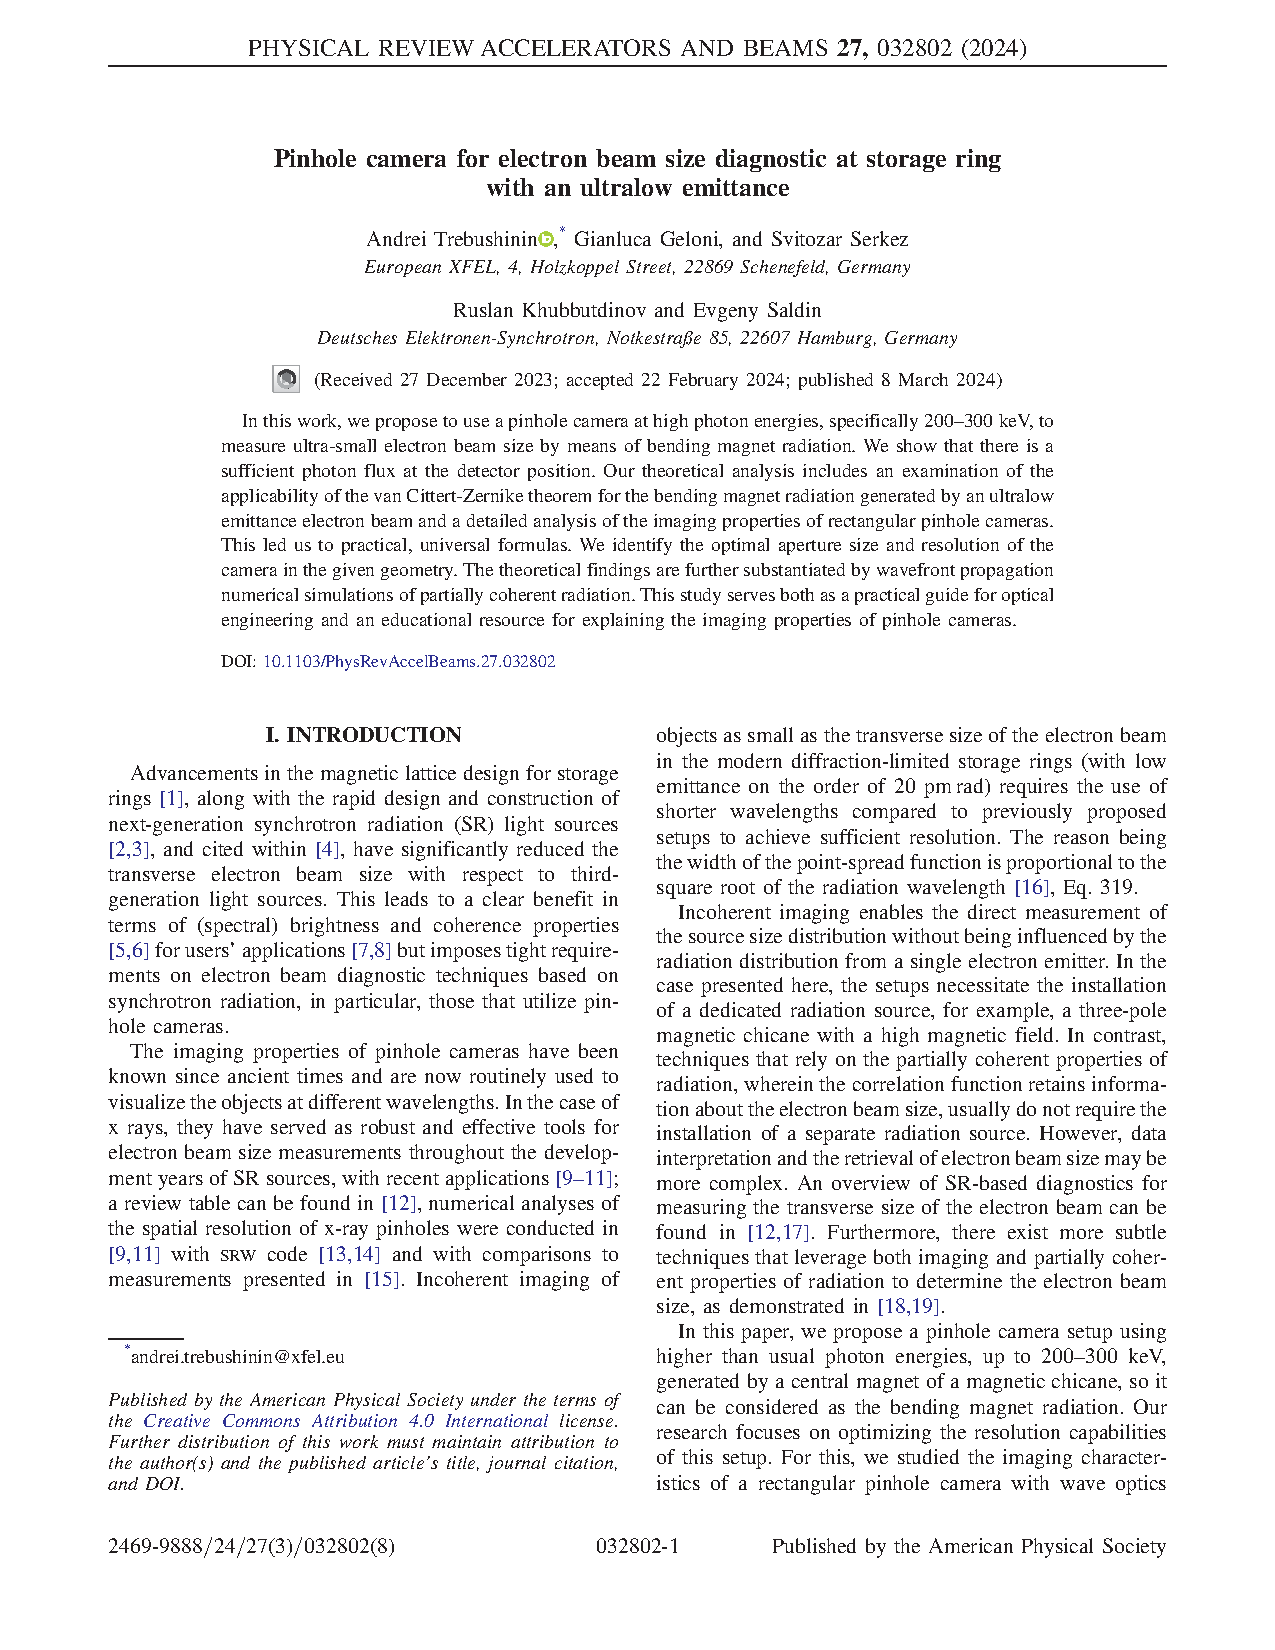
\includepdf[pages=-]{content/papers/pinhole.pdf}

    \subsection{Heuristic approach: quasi- homogeneous/stationary source}
        In the section~\ref{sec:Heuristic approach: homogeneous/stationary source} I have shown a method for simulating fully incoherent sources with a very broad divergence, here I would like to extend this heuristic to account for fine source divergence. If I take equation
        \begin{align}
            \bar{\phi}(\vec{k}) = \mathcal{F} \big[ \sqrt{I(\vec{r})} \mathcal{N}(\vec{r})\big](\vec{k})
        \end{align}
        where Fourier transform is encrypted in $\mathcal{F} \big[…\big]$ operator and multiply this field by the effective radiation divergence $\hat{I}(\vec{k})$ and take inverse Fourier transform I obtain the following expression:
        \begin{align}
            \phi(\vec{r}) = \mathcal{F}^{-1} \bigg[ \sqrt{\hat{I}(\vec{k})} \mathcal{F} \big[ \sqrt{I(\vec{r})} \mathcal{N}(\vec{r})\big](\vec{k})\bigg](\vec{r})
        \end{align}
        Writing the first integral explicitly and bringing the averaging sign inside:
        \begin{align}
            \langle \phi(\vec{r}_1) \phi^*(\vec{r}_2) \rangle =  
            \mathcal{F}^{-1} \bigg[  \sqrt{\hat{I}(\vec{k}_1)\hat{I}(\vec{k}_2)} \iint \limits_{-\infty}^{\infty}  \sqrt{I(\vec{r}'_1)I(\vec{r}'_1)} \big \langle\mathcal{N}(\vec{r}'_1)\mathcal{N}(\vec{r}'_2) \big \rangle e^{i (\vec{r}'_1\vec{k}_1 - \vec{r}'_2\vec{k}_2)}d\vec{r}'_1 d\vec{r}'_2  \bigg](\vec{r}_1, \vec{r}_2).
        \end{align}
        and taking this I obtain
        \begin{align}
            \langle \phi(\vec{r}_1) \phi^*(\vec{r}_2) \rangle =  
            \mathcal{F}^{-1} \bigg[  \sqrt{\hat{I}(\vec{k}_1)\hat{I}(\vec{k}_2)}  \iint \limits_{-\infty}^{\infty}  \sqrt{I(\vec{r}'_1)I(\vec{r}'_1)} \delta(\vec{r}'_1 - \vec{r}'_2) e^{i (\vec{r}'_1\vec{k}_1 - \vec{r}'_2\vec{k}_2)}d\vec{r}'_1 d\vec{r}'_2 \bigg](\vec{r}_1, \vec{r}_2).
        \end{align}
        integrating over one of the integrals and accounting for the filtering property of Dirac delta function:
        \begin{align}
            \langle \phi(\vec{r}_1) \phi^*(\vec{r}_2) \rangle =  
            \mathcal{F}^{-1} \bigg[ \sqrt{\hat{I}(\vec{k}_1)\hat{I}(\vec{k}_2)} \int \limits_{-\infty}^{\infty}  I(\vec{r}') e^{i (\vec{r}'(\vec{k}_1 - \vec{k}_2)}d\vec{r}'  \bigg](\vec{r}_1, \vec{r}_2).
        \end{align}
        again using part of the generalized van Cittert-Zernike theorem:
        \begin{align}
            \langle \phi(\vec{r}_1) \phi^*(\vec{r}_2) \rangle =  
            \iint \limits_{-\infty}^{\infty}  \sqrt{\hat{I}(\vec{k}_1)\hat{I}(\vec{k}_2)}\hat{g}(\Delta \vec{k}) e^{-i (\vec{r}_1\vec{k}_1 - \vec{r}_2\vec{k}_2)} d\vec{k}_1 d\vec{k}_2 = \cr 
            = \iint \limits_{-\infty}^{\infty} \langle \hat{E}(\vec{k}_1) \hat{E}^{*}(\vec{k}_2) \rangle  e^{-i (\vec{r}_1\vec{k}_1 - \vec{r}_2\vec{k}_2)} d\vec{k}_1 d\vec{k}_2 = \cr
            = \bigg\langle \int \limits_{-\infty}^{\infty} \hat{E}(\vec{k}_1) e^{-i \vec{r}_1\vec{k}_1} d\vec{k}_1 \int \limits_{-\infty}^{\infty} \hat{E}^{*}(\vec{k}_2) e^{i \vec{r}_2\vec{k}_2} d\vec{k}_2 \bigg\rangle = \langle E(\vec{r}_1)E^{*}(\vec{r}_2) \rangle.
        \end{align}
        It is very easy to show that intensity distributions and inverse space correlation also follows correct distributions.
        
    \subsection{SERVAL paper}
    \includepdf[pages=-]{content/papers/SERVAL.pdf}

    